% !TeX spellcheck = fr_FR
\documentclass[12pt, openany]{report}
\usepackage[utf8]{inputenc}
\usepackage[T1]{fontenc}
\usepackage[a4paper,left=2cm,right=2cm,top=2cm,bottom=2cm]{geometry}
\usepackage[frenchb]{babel}
\usepackage{libertine}
\usepackage[pdftex]{graphicx}
\usepackage{amssymb}
\usepackage{listings}
\usepackage{color}


\usepackage[colorlinks=true,linkcolor=red]{hyperref}
\usepackage[nottoc, notlof, notlot]{tocbibind}

\usepackage{cite}

\setlength{\parindent}{1cm}
\setlength{\parskip}{1ex plus 0.5ex minus 0.2ex}
\newcommand{\hsp}{\hspace{20pt}}
\newcommand{\HRule}{\rule{\linewidth}{0.5mm}}
\begin{document}

\begin{titlepage}
  \begin{sffamily}
  \begin{center}

    % Upper part of the page. The '~' is needed because \\
    % only works if a paragraph has started.
    
\includegraphics[scale=0.2]{Images/UMONS+txt.png}   ~\\[1.5cm]
    


    \HRule \\[0.4cm]
    { \huge \bfseries Projet de Software Evolution - JPacman\\[0.4cm] }
    \HRule \\[2cm]
    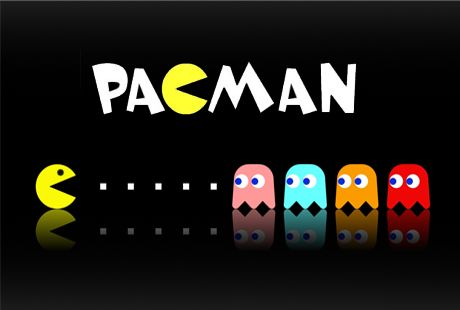
\includegraphics[scale=0.5]{Images/Pac-Man.jpg}~\\[1.5cm] 

    
    

    % Author and supervisor
    \begin{minipage}{0.4\textwidth}
      \begin{flushleft} \large
        \emph{Réalisateurs :\\} Damien \textsc{Legay}\\ Adrien \textsc{Coppens}\\ Nicolas \textsc{Leemans}\\
        
      \end{flushleft}
    \end{minipage}
    \begin{minipage}{0.4\textwidth}
      \begin{flushright} \large
        \emph{Enseignant :} M. Tom  \textsc{Mens}\\
        \emph{Date de remise : } 9 mai 2016\\
        \emph{Année d'étude : } Master 1
      \end{flushright}
    \end{minipage}

    \vfill

    % Bottom of the page
    {\large Année académique 2015 - 2016}
	
  \end{center}
  \end{sffamily}
\end{titlepage}




\newpage

	\renewcommand{\thesection}{\arabic{section}}
	\tableofcontents
	\newpage
	\setcounter{secnumdepth}{3}
	\setcounter{tocdepth}{4}
	

\section{Introduction}
%todo: uniformiser : \textit{Class#Method} ? (==javadoc) + préciser convention au début du rapport
Ce projet, effectué dans le cadre du cours de "Software Evolution" dispensé par le Professeur Tom Mens durant l'année académique 2015-2016, a pour but de mettre en pratique les concepts d'évolution logicielle vus au cours théorique. Il consiste à analyser et à étendre un projet en effectuant un contrôle de la qualité au travers de différentes métriques, le \textit{"refactoring"} du code source, ainsi que l'implémentation de nouvelles fonctionnalités. Le projet concerné s'appelle JPacman\footnote{https://github.com/SERG-Delft/jpacman-framework}. Il s'agit d'une implémentation très basique du jeu Pacman en Java, créé par l'équipe  du Professeur Arie van Deursen, Delft University of Technology (Pays-Bas).
 JPacman contient plusieurs simplifications par rapport au jeu Pac-Man original. Le jeu consiste à déplacer Pac-Man, un personnage qui, vu de profil, ressemble à un diagramme circulaire à l’intérieur d’un labyrinthe, afin de lui faire manger toutes les pac-gommes qui s’y trouvent en évitant d’être touché par des fantômes.
 
 Ce rapport s'organise en plusieurs chapitres : dans un premier chapitre, ...
 
\section{Extension du projet et ajout de tests unitaires pour cette extension }

\subsection{Extension du logiciel}

La première partie de ce projet consistait à étendre la version initiale de JPacman en ajoutant de nouvelles fonctionnalités et en suivant un processus de développement dirigé par les tests. De nouveaux tests unitaires ont donc été ajoutés pour chaque fonctionnalité afin de vérifier que le comportement initial du logiciel n’a pas été altéré. 

Chaque membre du groupe a donc implémenté une des fonctionnalités suivantes :
\begin{itemize}
\item L'implémentation d'un score (réalisée par Damien Legay)
\item L'implémentation d'une série de labyrinthes (réalisée par Adrien Coppens)
\item L'implémentation d'une intelligence artificielle pour pacman (réalisée par Nicolas Leemans)
\end{itemize}


\subsubsection{Fonctionnalité "Score"}\label{score}
Cette fontionalité requièrt l'implémentation de de deux sous-fonctionalités:

La première fonctionalité (Hall of Fame) consiste à maintenir une liste de hauts scores. Si un joueur dépasse l'un des dix meilleurs scores, son nom doit être inséré dans le Hall of Fame.
Ceci peut être réalisé de deux manières différentes: si le joueur est identifié, son nom de joueur sera automatiquement entré, si ce n'est pas le cas, il lui sera demandé de fournir un nom à la fin de la partie.
Le score du joueur est affecté par le nombre de gommes, phantômes et fruits consommés par Pacman, ainsi que par les hauts faits réalisés (voir ci-bas).

Lorsque la partie est terminée, le Hall of Fame est affiché et le joueur a l'option de le réinitialiser à ses valeurs par défaut. Pour éviter que celle-ci ne se fasse par mégarde, une confirmation est demandée.

La deuxième fonctionalité (Achievements) implique d'implémenter un système de gestion de hauts faits. 
Pour ce faire, un système de profils doit être mis en place, permettant au joueur la possibilité de s'identifier et ainsi réaliser des hauts faits qui sont mémorisés.
Ces hauts faits peuvent être accomplis sur plusieurs parties indépendentes.
Le joueur doit avoir la possibilité de visualiser les hauts faits qu'il a accompli avant de commençer à jouer, à la suite de quoi le jeu proposera de nouveaux haut faits à réaliser, au maximum de trois.
Lorsque le joueur obtient un haut fait, il reçoit un bonus de score.

Pour réaliser ces fonctionnalités, il a d'abord convenu d'associer à chaque élément pouvant être consommé par Pacman une valeur numérique à ajouter au score, même pour les éléments que Pacman ne peut pas manger à ce stade puisque dépendants de fonctionnalités non implémentées (fruits, supergomme pour manger les phantômes).
Ces valeurs sont localisées dans les classes \mbox{\textit{LevelFactory}} (gommes et fruits) et \mbox{\textit{Ghost}} (phantômes).

Ensuite, un système de Hall of Fame a été mis en place à l'aide de la classe \mbox{\textit{HallOfFame}} qui offre les services suivants:

\begin{enumerate}
\item La méthode \mbox{\textit{HallOfFame\#handleHoF()}} se charge de mettre à jour le Hall of Fame si nécessaire, c'est à dire si le score du joueur excède l'un des scores sauvegardés dans le fichier \mbox{\textit{resources\\HoF.txt}}, et de l'afficher qu'il ait été mis à jour ou non.
\item La méthode \mbox{\textit{HallOfFame\#resetHoF()}}, quant à elle, a pour rôle de réinitialiser le Hall of Fame aux valeurs par défaut telles que définies dans le fichier \mbox{\textit{resources\\DefaultHoF.txt}}.
\end{enumerate}

\begin{figure}[h]
	\centering
	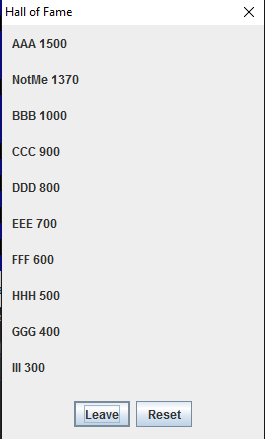
\includegraphics[width=6cm]{Images/HoF.png}
	\caption{\label{hof} Le Hall of Fame après que le joueur "NotMe" a terminé une partie}
\end{figure}


Enfin, un système de gestion des hauts faits a été réalisé. Pour cela, il a été nécessaire de mettre un oeuvre un système d'authentification du joueur.
Ce système se repose sur les éléments qui voici:

\begin{enumerate}
\item Le fichier \mbox{\textit{resources\\login.txt}}, dans lequel sont stockés les identifiants et mots de passes (non en clair) des joueurs ;
\item Le répertoire \mbox{\textit{resources\\profiles\\}}, qui contient les profils des joueurs ayant créé un compte.
Le format des fichiers .prf contenus dans ce répertoire est tel que suit: 
\begin{itemize}
\item La première ligne contient des informations diverses : score maximal atteint par le joueur, nombre fois qu'il a été tué par tel phantôme, niveau maximum que le joueur a complété,...
\item Les lignes suivantes contiennent le nom d'un haut fait accompli par le joueur.
\end{itemize}
\item La méthode \mbox{\textit{IdentifiedPlayer\#createNewPlayer()}}, qui permet à un joueur de créér un nouveau profil joueur, et, si besoin est, le répertoire ci-dessus ;
\item La méthode \mbox{\textit{IdentifiedPlayer\#authenticate()}}, qui vérifie que l'identifiant et le mot de passe entrés par le joueur correspondent bien à des données situées dans \mbox{\textit{resources\\login.txt}} et, si le joueur le désire, affiche les hauts faits qu'il a déjà obtenus ;
\item La méthode \mbox{\textit{IdentifiedPlayer\#addAchievement()}}, servant à ajouter un haut fait que le joueur a obtenu dans son fichier profil, si celui-ci ne s' y trouve déjà ;
\item La méthode \mbox{\textit{IdentifiedPlayer\#saveScore()}}, qui met à jour le score maximal du joueur et lui accorde les hauts faits liés à celui-ci ;
\item La méthode \mbox{\textit{IdentifiedPlayer\#killedBy()}}, mettant à jour les informations liées au fait de s'être fait tuer par un phantôme et affectant les hauts faits correspondants ;
\item La méthode \mbox{\textit{IdentifiedPlayer\#levelCompleted()}} en fait de même pour le niveau maximal atteint ;
\item La méthode \mbox{\textit{IdentifiedPlayer\#displayProfileStats()}}, qui affiche les informations concernant le joueur, s'il est identifié, et lui propose d'en accomplir d'autres, s'il n'a pas accompli tous les hauts faits disponibles ;
\item La classe utilitaire \mbox{\textit{FileChecker}} qui effectue certaines opérations de vérification sur les fichiers susnommés ;
\item L'énumération \mbox{\textit{Achievement}} dans laquelle sont stockés les hauts faits, le score qu'ils accordent lorsqu'accomplis, une description définissant comment les obtenir et le haut fait à recommender après leur obtention.
\end{enumerate}


\subsubsection{Fonctionnalité "Série de labyrinthes"}
Les ajouts à effectuer pour cette extension sont :
\begin{enumerate}
	\item Système de vies pour Pac-man, au nombre de 3 initialement,
	\item Gain d'une vie supplémentaire tous les 10000 points,
	\item Téléportation de Pac-man lorsqu'il est tué par un fantôme (et qu'il lui reste au moins une vie),
	\item Ajouts d'autres niveaux en préservant la vie et le score de Pac-man lors du passage au niveau suivant (ce qui se produit lorsque toutes les gommes ont été ramassées),
	\item Sauvegarde du \og meilleur \fg \, niveau atteint pour pouvoir, par la suite, débuter directement à un niveau précédemment accédé.
\end{enumerate} 

$(1)$ a simplement été réalisé par l'ajout d'un champ \mbox{\textit{lives}} dans la classe \mbox{\textit{Player}} et en faisant en sorte que, lors de la collision avec un fantôme, Pac-man perde une vie plutôt que de mourir (appel à \mbox{\textit{Player\#loseLife}} plutôt qu'à \mbox{\textit{Player\#setAlive(false)}}).

De la même manière, la réalisation de $(2)$ a pu se faire rapidement, en ajoutant une méthode \mbox{\textit{Player\#checkNewLifeThreshold(int)}}, appelée à chaque fois que le joueur reçoit des points. Cette méthode se contente de vérifier si le seuil a été dépassé et ajoute une vie au joueur le cas échéant.

L'ajout $(3)$ a demandé plus de réflexion quant à la manière de l'implémenter. En effet, pour permettre une téléportation \og safe \fg , il est nécessaire d'avoir connaissance du niveau (le \mbox{\textit{Board}}), alors que le joueur est, en l'état, le seul à être au courant de sa mort.

Il a été choisi ici d'implémenter un design pattern \mbox{\textit{Observer}}, via une interface \mbox{\textit{PlayerListener}}, qui ne contient qu'une méthode \mbox{\textit{onPlayerLoseLife(Player)}} mais qui pourrait être facilement étendue (pour par exemple permettre l'affichage d'une notification lorsque le joueur reçoit une vie).

Via l'implémentation de \mbox{\textit{PlayerListener}}, \mbox{\textit{Level}} est capable de réagir à la mort du joueur et, puisqu'il possède une référence vers le \mbox{\textit{Board}}, de le téléporter. L'énoncé demande une téléportation \textit{aléatoire} à une distance de 4 cases de tout fantôme, il sera fait utilisation de la distance Manhattan\footnote{\url{https://en.wiktionary.org/wiki/Manhattan_distance}}.

Lorsque Pac-man meurt, une liste des cases \og possibles \fg \, est récupérée via la méthode \mbox{\textit{Level\#getPossibleSquares()}} et le joueur est effectivement transporté aléatoirement sur l'une de celles-ci. Afin de déterminer si une case est \og possible \fg , on s'assure qu'elle soit accessible (qu'elle ne corresponde pas à un mur par exemple) et \og safe \fg , c'est-à-dire qu'aucun fantôme ne soit à portée.

Pour ce faire, pour toute case accessible, on vérifie les occupants des cases \og voisines \fg \, en s'assurant qu'elles ne contiennent pas de fantôme. En réalité, puisque les cases situées à une distance Manhattan d'une case donnée forment une sorte de losange, on itère sur le rectangle des cases situées à une distance horizontale et verticale inférieure à 4, en filtrant ensuite les cases trop éloignées en distance Manhattan. 

Cette situation est représentée à la figure \ref{manhattan}, dans laquelle on s'intéresse à une distance Manhattan de 4 cases à partir de la case {\color{blue}{bleue}}. Les cases à une telle distance sont en {\color{green}{vert}} alors que les cases filtrées sont en {\color{red}{rouge}} (les cases noires ne sont pas du tout prises en compte).
\begin{figure}[h]
	\centering
	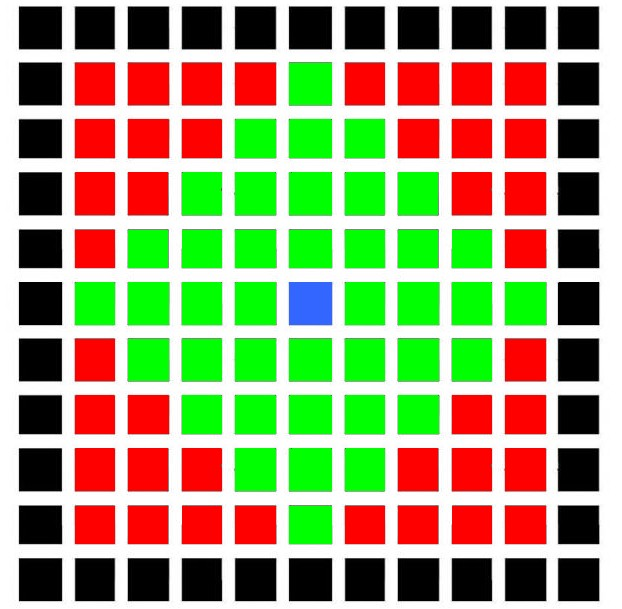
\includegraphics[width=6cm]{Images/manhattan.jpg}
	\caption{\label{manhattan} Cases à une distance Manhattan de 4}
\end{figure}

$(4)$ était également problématique puisque \mbox{\textit{Level}} et \mbox{\textit{Game}} étaient les seuls à être au courant de la réussite d'un niveau, alors que les méthodes permettant le chargement d'un niveau (via \mbox{\textit{MapParser}}) se trouvaient dans \mbox{\textit{Launcher}}. 

La solution logique semblait être de déplacer les méthodes appelant \mbox{\textit{MapParser}} de \mbox{\textit{Launcher}} vers \mbox{\textit{Game}} mais il a été décidé d'attendre la fusion des différentes extensions individuelles pour réaliser ce changement. Nous voulions en réalité éviter les conflits potentiels lors de la fusion puisque ce \og transfert \fg de méthodes demande un nombre important de modifications dans le code d'origine. En attendant la fusion, on a donc simplement fait en sorte que \mbox{\textit{Game}} aie la référence vers une instance de \mbox{\textit{Launcher}}.

$(5)$ posait lui aussi quelques difficultés, non pas sur sa réalisation en soi mais bien sur la redondance potentielle et la future intégration avec le système de profil de l'extension \og Score \fg \, (section \ref{score}) . 

Pour cette fonctionnalité, il a été choisi de simuler l'authentification en respectant des conventions de nommage communes. On fournira ici les méthodes permettant, une fois qu'a été récupéré le niveau maximum atteint par un joueur, d'ajouter des boutons de sélection/chargement de niveau tout en réinitialisant le score et les vies du joueur.

Pour les ajouts $(4)$ et $(5)$, il a été nécessaire d'ajouter des fichiers de niveaux supplémentaires. Puisque la démarche était fastidieuse, une fonctionnalité \og bonus \fg \, a été implémentée : la génération de fichiers de niveaux au format Pac-man à partir d'une image. \label{map_generator_txt}

En effet, en attribuant une couleur à chaque type d'élément du jeu,  une image peut être convertie en un fichier texte équivalent et \og lisible \fg \, par \mbox{\textit{MapParser}}. Cela permet de créer des niveaux rapidement avec n'importe quel logiciel d'édition d'image puisqu'ils permettent d'utiliser des fonctionnalités comme le \og remplissage \fg d'une zone, qui évite donc d'entrer le même caractère un grand nombre de fois (on obtient également un rendu visuel plus clair que le fichier texte équivalent). 

La figure \ref{map_generator_img} montre un exemple de résultat de conversion d'une image en son niveau équivalent dans JPacman.
\begin{figure}[h]
	\centering
	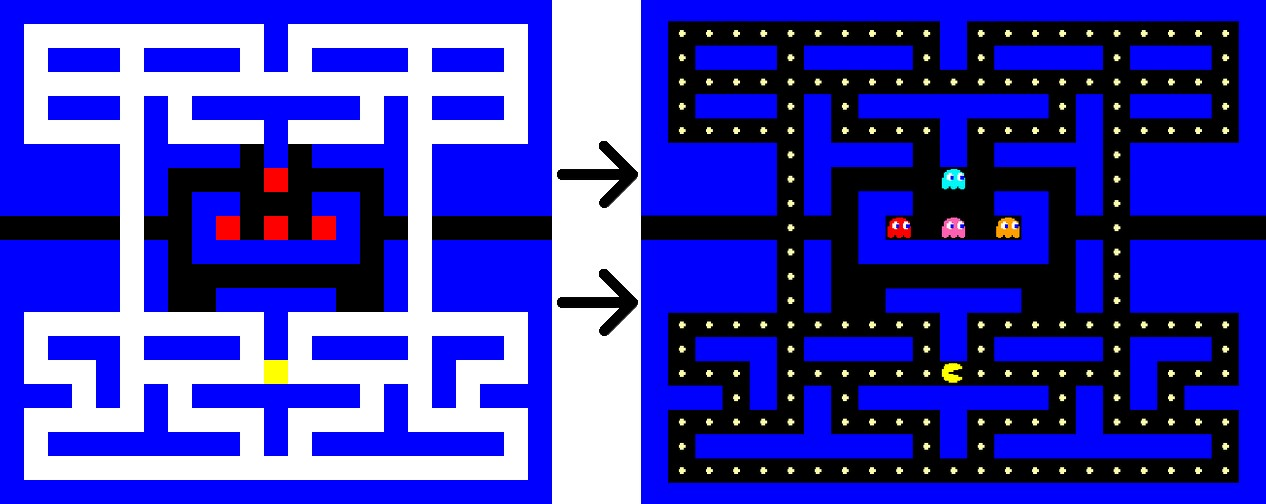
\includegraphics[width=13cm]{Images/mapgenerator.jpg}
	\caption{\label{map_generator_img} Génération d'un niveau à partir d'une image}
\end{figure}

\subsubsection{Fonctionnalité "IA pour Pacman"}

L'objectif de cette fonctionnalité est d'intégrer au code existant une intelligence artificielle pour Pacman afin qu'il puisse jouer de façon autonome tout en optimisant son score. En début de partie, le joueur doit pouvoir choisir entre contrôler Pacman manuellement ou être un spectateur passif de la partie en choisissant l'intelligence artificielle qui contrôlera Pacman à la place du joueur. Pour mettre en place cela, il a été recommandé d'utiliser un design pattern nommé "Strategy". Le design pattern "Strategy" consiste à définir un comportement (appelée "strategie") qui va permettre de différencier l'utilisation entre l'IA ou le contrôle manuel. Ce design pattern offre également une flexibilité pour modifier la stratégie suivie très facilement.

Les ajouts à effectuer pour cette extension sont les suivantes :
\begin{enumerate}
	\item Déplacement continu de Pacman,
	\item Intelligence artificielle contrôlant Pacman et qui optimise son score,
	\item Différents comportement pour Pacman,
	\item Choix du mode de jeu en début de partie (contrôle du Pacman ou spectateur passif)
	\item Extension possible et facile de nouvelles stratégies en bannissant tout type de triche \\
	
\end{enumerate} 

L'ajout de la fonctionnalité $(1)$ a été réalisé en ajoutant une méthode \mbox{\textit{Game\#continousMovement()}}, appelée à chaque fois que le joueur appuie sur une touche directionnelle, qui va manipuler un unique \textit{thread} qui va appeler, de façon périodique, la méthode \mbox{\textit{Game\#move()}}. A chaque fois que le joueur appuiera sur une touche directionnelle, la méthode \mbox{\textit{Game\#continousMovement()}} va tester si la case voulant être accédée par le joueur est accessible à Pacman. Si c'est le cas, la tâche courante du \textit{thread} sera mis à jour et Pacman avancera dans une nouvelle direction. Par contre, si ce n'est pas le cas, l'instruction sera simplement ignorée et Pacman conservera son ancienne direction. 

Remarque : Pour cette fonctionnalité, il est supposé qu'il suffit d'appuyer une fois sur la touche pour conduire le Pacman dans la direction désirée ce qui veut dire que l'appui abusif d'une même touche directionnelle provoquera un ralentissement voir un arrêt du Pacman.

L'ajout de la fonctionnalité $(2)$ concerne l'implémentation d'un intelligence artificielle manipulant Pacman et qui optimise son score. Le comportement de l'IA est défini dans la classe\\
 \mbox{\textit{PacManhatanAI\#nextMove()}}. Ce comportement est calculé grâce à une recherche en largeur qui permet de déterminer la gomme la plus proche (\mbox{\textit{PacManhatanAI\#bfsNearestSafetyPelletSquare()}}). Une fois la case déterminée, il a été choisi d'utiliser un algorithme de type $A^*$ (classe \mbox{\textit{AStarPath}}
) afin de déterminer le chemin le plus court et le plus sûr en appliquant un système de poids aux cases de la carte en fonction de la présence d'une gomme, d'un fantôme ou de la proximité d'un fantôme. L'algorithme $A^*$ a été implémenté grâce à une classe template open-source fournie par Giuseppe Scrivano\footnote{http://a-star.googlecode.com/svn/trunk/java/AStar.java}
(classe \mbox{\textit{AStar}}
). Cet algorithme permet de se focaliser sur la direction du chemin en privilégiant toute direction se rapprochant de la destination par opposition à l'algorithme Dijkstra qui calcule tous les chemins possibles, ce qui est en général moins performant que l'algorithme $A^*$ car celui-ci évite autant que possible les chemins s'éloignant de la destination. Une fois un chemin déterminé, il est stocké sous forme de direction qui sera suivie par Pacman si aucun danger ne se présente (\mbox{\textit{PacManhatanAI\#convertPathToDirection()}}
). Avant de choisir le prochain mouvement, l'IA détermine si Pacman est dans une zone sûre ou non (\mbox{\textit{PacManhatanAI\#bfsNearestSafetySquare()}}
). S'il est trop proche d'un fantôme, alors l'IA choisit de prendre une nouvelle destination qui est la case sûre la plus proche. Le seuil initial pour déterminer si Pacman est proche d'un fantôme est de 14 cases, dans l'implémentation, ce qui permet de jouer un début de partie de façon très sûre. Ce seuil diminuera au cours de la partie en fonction des gommes restantes pour se focaliser sur les gommes en fin de partie (\mbox{\textit{PacManhatanAI\#updatePacmanbehaviour()}}
). Le fait d'avoir un seuil dynamique offre de bons résultats en pratique. Une fois que Pacman est dans une zone sûre, il recommence à chasser les gommes. Pour finir, pour avoir la certitude que l'IA renvoie une direction à suivre peu importe où le Pacman se trouve sur le plateau de jeu, une méthode \mbox{\textit{PacManhatanAI\#hurryMove()}}
a été implémentée pour déterminer une direction imposée qui mène à une case accessible dans le cas où aucune autre direction n'a pu être choisie. Bien que ce cas de figure n'apparaît jamais en pratique, il a été pensé en vue de l'intégration d'autres fonctionnalités comme la téléportation (voir 2.1.2 Fonctionnalité "Série de labyrinthes").

Remarque : On peut facilement constater que l'IA se base sur la carte existante et ne passe pas par la construction d'un graphe, ce qui évite de devoir reconstruire le graphe à chaque action, ce qui pourrait être plus gourmand en performances. De plus, ce choix de comportement a été effectué en prenant en considération qu'un autre membre du projet travaillait sur un système de niveaux différents et donc les stratégies définies sur certains sites pour le jeu Pacman ne pouvaient pas être appliquées sur d'autres types de cartes. Ne pouvant pas implémenter une stratégie gagnante, il a été préféré d'appliquer une stratégie qui joue de façon la plus sûre possible tout en essayant de finir le niveau. 



L'ajout de la fonctionnalité $(3)$ a été réalisé en utilisant le design pattern "Strategy" qui va permettre d'établir différents comportement pour Pacman, sous forme de stratégie, et de choisir un type de comportement en début de partie. En ce qui concerne son implémentation, une stratégie est définie par une classe abstraite \mbox{\textit{PacmanStrategy}} qui définit certains attributs utiles aux stratégies, une méthode \mbox{\textit{PacmanStrategy\#getTypeStrategy()}} qui retourne le type de la stratégie (contrôle du Pacman par le joueur ou par une AI), une méthode \mbox{\textit{PacmanStrategy\#executeStrategy()}} qui permet d'attribuer les touches au joueur dans le cas où la stratégie choisie est le contrôle du Pacman par le joueur et une méthode \mbox{\textit{PacmanStrategy\#nextMove()}} qui retourne la prochaine direction à suivre. Une classe intermédiaire "AIStrategy" est définie pour manipuler plus facilement les stratégies où Pacman est conduit par une intelligence artificielle. Cette classe définit également des attributs plus spécifiques qui sont uniquement utiles aux stratégies de type IA pour déterminer la prochaine direction à suivre lors d'une partie en cours.

Au niveau des stratégies implémentées, la classe \mbox{\textit{HumanControllerStrategy}} représente la stratégie où le Pacman est contrôlé par un joueur humain. Le but de cette stratégie étant seulement de définir les touches de contrôle et de les attribuer au joueur pour qu'il puisse manipuler le Pacman lors d'une partie. La classe \mbox{\textit{PacManhatanAI}} représente la classe définissant le comportement de l'IA expliqué au point $(2)$.



La fonctionnalité $(4)$ a été mise en place pour que le joueur puisse choisir quelle stratégie appliquer, c'est-à-dire quel comportement attribué au Pacman pour une partie complète. Afin de laisser le joueur choisir, une fenêtre de sélection est affichée au lancement du jeu et permet de déterminer la stratégie qui sera appliquée pour toute une partie (la stratégie ne pourra pas changer lors d'un jeu en cours). Une fois que le joueur aura choisi une stratégie, il lui suffit de lancer la partie pour que celle-ci définisse un comportement spécifique à Pacman.

La classe \mbox{\textit{Level}} est utilisée pour implémenter les méthodes liées à la gestion des stratégies durant une partie. En effet, cette classe semblait la plus adéquate car elle correspond au niveau courant qui contient toutes les informations dont les stratégies ont besoin. Il est important de signaler qu'après l'intégration de toutes les fonctionnalités, les méthodes liées à la gestion des intelligences artificielles (joueur et fantômes) ont été déplacé dans une nouvelle classe \mbox{\textit{AILevel}} (voir Refactorings...). Les méthodes \mbox{\textit{Level\#start()}} et \mbox{\textit{Level\#stop()}} permettent d'exécuter ou d'arrêter l'action spécifique définie selon le type de stratégie choisie. Dans le cas d'une stratégie où le joueur est un humain, l'attribution des touches sera appliquée au joueur. Tandis que dans le cas d'une stratégie d'intelligence artificielle, la méthode \mbox{\textit{Level\#startAIStrategy()}} est appelée pour lancer un unique \textit{thread} qui va de façon périodique attribuer une direction à suivre au Pacman et appliquer un mouvement dans cette direction. Une nouvelle direction devant être calculée uniquement lorsque le Pacman se trouve à une intersection, un test a été ajouté pour définir cette situation. Dans le cas où le Pacman ne se trouve pas à une intersection, l'action effectuée correspondra à l'action courante (ancien mouvement). Le comportement du \textit{thread} pour la gestion des intelligences artificielles est défini dans la méthode \mbox{\textit{Level/PlayerMoveTask\#run()}}


La fonctionnalité $(5)$ concerne le fait de pouvoir ajouter facilement des stratégies définissant de nouveaux comportements pour Pacman sans pour autant autoriser des stratégies qui trichent. Tout d'abord, l'implémentation des stratégies a été réfléchie pour que l'ajout de nouvelles stratégies soient faciles. En effet, comme expliqué en $(3)$, les classes abstraites \mbox{\textit{PacmanStrategy}} et \mbox{\textit{AIStrategy}} permettent de manipuler plus facilement les différents types de stratégies possibles en définissant les informations et les méthodes nécessaires aux différentes stratégies. L'implémentation d'une nouvelle stratégie se fera donc par la création d'une nouvelle classe, implémentant le comportement de la stratégie, et qui étendra l'une de ces deux classes en fonction de son type. Pour les stratégies d'intelligence artificielle, la nouvelle classe devra implémenter une méthode \mbox{\textit{nextMove()}} qui retournera la prochaine direction à suivre par Pacman. Ensuite, pour interdire tout type de triche, les attributs, se trouvant dans les classes mères \mbox{\textit{PacmanStrategy}} et \mbox{\textit{AIStrategy}}, qui représentent les caractéristiques du niveau en cours lors d'une partie, ont été implémenté avec le mot clé "final" et uniquement des méthodes d'accesseurs. Ainsi, comme les stratégies étendent ces classes, ils auront accès à ces attributs grâce aux méthodes accesseurs mais ne pourront en aucun cas modifier ces valeurs. En ne permettant pas de modifier les données du jeu, les stratégies ne pourront pas tricher dans la manipulation des données lors du calcul de la prochaine direction à suivre.


\section{Refactorings avant analyse}
%todo: ce qui était prévu juste après merge, qu'on avait laissé tel quel ds les parties individuelles pr éviter au maximum les conflits lors de l'intégration des PR

\subsection{Fusion des tests sur \og Player \fg}
%Des tests avaient été effectués par 2 d’entre nous et lors de la fusion, nous avions simplement fusionné ceux-ci en ignorant la redondance de variables d’instances. L’un des 2 tests n’utilisant pas les \og mocks \fg, une légère adaptation a été nécessaire pour que le mock de fantôme retourne une valeur lors de l’appel à \og Ghost#getIdentity() \fg.
\subsection{Déplacement de la variable retenant le niveau courant de \og Level \fg vers \og Game \fg}
%Plus logique et évite un problème de \og feature envy \fg 
\subsection{Déplacement des méthodes concernant le \og map parser \fg de \og Launcher \fg vers \og Game \fg}
%Plus logique et évite que \og Game \fg doive avoir une référence vers le \og Launcher \fg qui l’a créé (pour pouvoir charger le niveau suivant en cas de \og victoire \fg)
%A nécessité de passer des méthodes/variables en \og static \fg (une partie des accesseurs aux \og Factories \fg de \og Launcher \fg puisque \og MapParser \fg en a besoin) mais cela reste logique puisque ces méthodes/variables sont en effet uniques au runtime.









\section{Analyse de la qualité du code source}

Dans ce chapitre, nous allons comparer la qualité du code source qui intègre toutes les extensions individuelles avec la qualité du code source de la version de départ de JPacman. Pour pouvoir effectuer cette comparaison, il va, tout d'abord, falloir effectuer des analyses sur la qualité du code source des deux versions en utilisant différents types d'analyses et de techniques. Pour effectuer cette analyse, nous ferons appel à plusieurs outils d'analyse de qualité que nous détaillerons par la suite. Cette phase d'analyse se déroulera en trois étapes : une analyse statique et dynamique du code ainsi qu'une analyse de la qualité par plusieurs métriques logicielles qui peuvent aider à déceler de mauvaises pratiques. 

\section{Analyse statique}
\subsection{Code dupliqué}
Puisque nous utilisons tous les 3 IntelliJ IDEA, l'outil intégré a été utilisé dans un premier temps. La figure \ref{duplicate} montre les résultats obtenus via cette analyse.
On peut noter que les détections ayant un \og coût \fg \, inférieur à $\sim$20 ne sont pas réellement préoccupantes. Pour exemple, les lignes suivantes, extraites de \textit{SquareCoordinateTest}, sont considérées comme dupliquées par l'outil avec un score de 10 :
\begin{lstlisting}[language=java]
assertEquals(square.getSquareAt(Direction.WEST).getY(), 15);
assertEquals(square.getSquareAt(Direction.EAST).getY(), 15);
\end{lstlisting}
Il s'agit en effet de 2 lignes très similaires mais il ne nous a pas semblé intéressant de supprimer ce type de duplicat. 
%todo: actions en réaction aux duplicats évitables et significatifs (outil intellij avec coût > 25? résultats de CPD?)
Dans un second temps, nous avons analysé le code via \textit{CPD} inclus dans \textit{PMD} et qui était utilisé dans la suite de rapports à générer par \textit{Maven}. Le seul dupliqué signalé par cet outil concerne la classe \textit{AStarPathTest} pour laquelle les méthodes \textit{hTest} et \textit{gTest} contiennent en effet toutes deux ce bloc de code :
\begin{lstlisting}[language=java]
final AStarPath aStarPath = new AStarPath(game);

assertNotNull(aStarPath);
final Player player = game.getPlayers().get(0);
final Square square = player.getSquare();

assertNotNull(player);
assertNotNull(square);

final Square origin = player.getSquare();
final Square destination = player.getSquare().getSquareAt(Direction.EAST);
final Square destination2 = player.getSquare().getSquareAt(Direction.EAST).getSquareAt(Direction.EAST);

final Square destination3 = player.getSquare().getSquareAt(Direction.WEST);
final Square destination4 = player.getSquare().getSquareAt(Direction.WEST).getSquareAt(Direction.WEST);
\end{lstlisting}
%todo: nicolas: action entreprise (extract method?)

\begin{figure}[h]
	\centering
	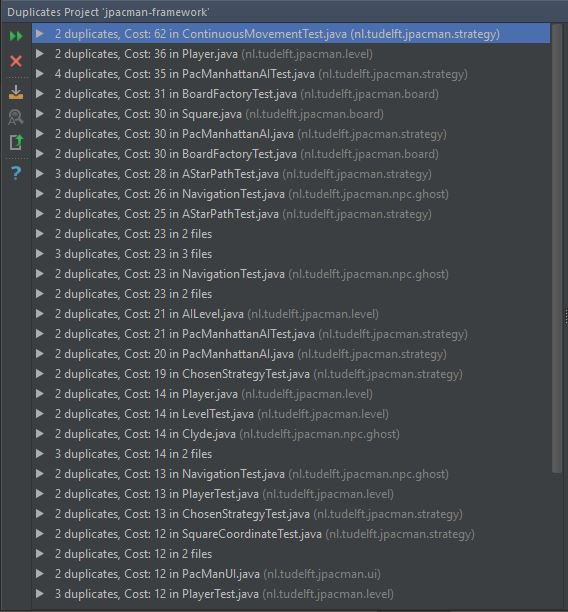
\includegraphics{Images/duplicate_analysis.JPG}
	\caption{\label{duplicate} Recherche de code dupliqué via l'outil intégré à \textit{IntelliJ IDEA}}
\end{figure}

\subsection{Audit de code}
\subsubsection{CheckStyle}
Egalement intégré dans la suite d'analyses à effectuer via \textit{Maven}, \textit{CheckStyle} a été utilisé avec le \og ruleset \fg \, présent dans la version du code d'origine.
Aucune erreur n'a été détectée mais de nombreux \og warnings \fg \, sont cependant présents (plus de 500). Par ordre de nombre de \og violations \fg :
\begin{itemize}
	\item 148 violations de type \textit{JavadocStyle} : en réalité toutes des \og First sentence should end with a period. \fg $\rightarrow$ réglé. 
	\item 110 violations de type \textit{MagicNumber} $\rightarrow$ constantes extraites là où cela avait du sens, sauf pour les tests où un tel refactoring nous semblait inutile, nous avons donc supprimé les \og warnings \fg \, pour ceux-ci.
	\item 104 violations de type \textit{LineLength} $\rightarrow$ retours à la ligne là où c'était nécessaire.
	\item 63 violations de type \textit{NeedBraces} $\rightarrow$ bien que nous ne soyons pas tous d'accord sur la valeur ajoutée d'une telle convention, nous avons ajouté les crochets là où \textit{CheckStyle} le demandait.
	\item 35 violations de type \textit{AvoidStarImport} $\rightarrow$ encore une fois désactivés car nous utilisons la fonction \og optimize imports \fg \, d'\textit{IntelliJ IDEA} qui regroupe parfois des imports en un unique via cette notation.
	\item Des violations relatives à des éléments de javadoc manquants $\rightarrow$ ajoutés.
	\item Des violations relatives à des tableaux déclarés à la \og mode C \fg \, plutôt qu' à la \og mode Java \fg $\rightarrow$ modifiés.
	\item D'autres violations plus \og isolées \fg \, non reprises ici.
\end{itemize}

\subsubsection{IntelliJ Code inspection}
\paragraph{IntelliJ dit que la condition impliquant QUICK\_WIN est \og pointless \fg} 
%Puisque la variable mise à true ou false dans le code, c’est effectivement le cas sur le code compilé, pas dans le code source puisqu’on veut pouvoir le changer. Note qu’on pourrait aussi permettre de set ça en paramètre au lancement du prog (option type \og --quick \fg)
\paragraph{Mineures altérations diverses}
\begin{itemize}
	\item La variable de classe \og Level \fg{} dans \mbox{\textit{SinglePlayerTest}} fut convertie en variable locale,
	\item 4 booléens n'avaient aucun intérêt et furent donc ôtés,
	\item 6 paramètres avaient toujours la même valeur et furent donc remplaçés par celle-ci,
	\item 14 accès furent rendus plus restrictifs,
	\item La valeur de retour de la méthode \mbox{\textit{Level/PlayerMoveTask\#run()}} n'était pas utilisée et cette méthode a donc été convertie en \og void \fg{},
	\item 8 variables ont été déclarées \og final \fg{},
	\item 11 éléments étaient reportés inutilisés, ceux qui n'avaient pas d'usage ont été enlevés (les autres sont suite à la gestion du score de fonctionnalités non implémentées),
	\item Les 5 constantes dans \mbox{\textit{SinglePlayerTest\#constantTest()}} étaient accédées par référence d' instance, elles sont maintenant accédées par référence de classe, 
	\item 7 types anonymes ont été remplaçés par des expressions lambda,
	\item 3 déclarations de type explicites furent remplaçés par \og <> \fg{} dans le contexte de listes,
	\item 2 boucles de type \og for each \fg{} furent remplaçées par des flux,
	\item Intellij a soulévé 3 erreurs dans la Javadoc, qui furent corrigées,
	\item 6 \og asserts \fg{} étaient toujours vrais, ils ne le sont plus.
\end{itemize}
\paragraph{Dans le code de base, beaucoup de \og warnings \fg sur des \og problèmes de modernité \fg}
%for indexé plutôt que foreach, méthode anonyme classique plutôt que lambda, etc


\subsubsection{PMD}
\paragraph{Déplacement des méthodes liées à la récupération des cases \og safe \fg pour téléporter le joueur de Level vers Board}
%Plus logique et évite un problème de \og feature envy \fg desdites méthodes
\paragraph{Problème détecté par PMD : Level == godclass, PacManhatanAI et Player aussi}
%Signifie que :
%1.	Level a une \og cohésion interne \fg faible, nous sommes en effet très loin du seuil de 1/3 mais cela devait également être le cas dans la version de base
%2.	Level accède à des attributs appartenant à trop de classes étrangères, encore une fois, peu de changements à ce niveau là par rapport à la version de base
%3.	Level est \og trop complexe par rapport à sa taille \fg : le problème ici semble venir de PMD qui, d’après la règle définie sur https://pmd.github.io/pmd-5.4.1/pmd-java/xref/net/sourceforge/pmd/lang/java/rule/design/GodClassRule.html attribue effectivement une valeur de complexité mais à aucun moment ne prend en compte la \og taille \fg de la classe.
%Etant donné que Level comprend beaucoup de méthodes, la complexité est naturellement élevée.

%Player:
% Regroupait l'implémentation de deux fonctionnalités séparées (score & labyrinthe) en plus des services de base. -> Comportement lié à la fonctionnalité "score" déplaçé dans la classe descendante "IdentifiedPlayer" et de méthodes de vérification de contenu de fichiers verfs "FileChecker.

A ce jour, il ne reste plus de \og god class \fg() dans l'implémentation.


\paragraph{Taille de code}
Deux classes (\mbox{\textit{Player}} et \mbox{\textit{Launcher}}) avaient trop de méthodes, donc certaines furent déplaçées ou intégrées à une méthode appelante lorsque possible.

La classe (\mbox{\textit{PacManhattanAI}} et \mbox{\textit{PacManhattanAI}}) et la méthode \mbox{\textit{PacManhattanAI\#BFSNearestPelletSquare()}}) avaient une complexité cyclomatique trop élevée, elles ont donc été l'object de \og refactorings \fg() afin de réduire celle-ci.

\paragraph{Loi de Demeter}
PMD détecten nombreuses violations de celle loi, mais beaucoup d'entre elles viennent du code originel et la vaste majorité relèvent d'appels à des librairies standard Java, il nous a donc paru que la détection de PMD était inadéquate à ce niveau.
Pour ce qui est des autres violations, le code existant force largement à les commettre.

\paragraph{Avertissements mineurs}
\begin{itemize}
	\item Deux \og if \fg{} imbriqués dans \mbox{\textit{PlayerMoveTask\#run()}} furent intégrés en un seul,
	\item 9 Arraylists furent convertis en List et une Hasmap en Map,
	\item 4 \og varargs \fg{} furent introduits là où c'était possible,
	\item 5 déclarations d'attributs de classe furent déplaçés à la tête de leur classe,
	\item 15 \og assert \fg{} furent modifiés pour éviter la surdépendance à \og assertTrue() \fg{},
	\item 251 messages d'erreur furent ajoutés aux \og assert \fg{} qui en étaient privés,
	\item Certaines variables au nom trop court furent renommées, d' autres non (variable à l'étendue fort restreinte ou correspondant à des coordonnées cartésiennes),
	\item Des méthodes, variables, classes et constantes ont été renommées pour correspondre aux conventions du langage,
	\item De nombreuses variables et paramètres furent déclarés \og final \fg{},
	\item L'initialisation superflue de \mbox{\textit{PlayerMoveTask\#finished}} a été ôtée.
\end{itemize}

\subsubsection{FindBugs}
%Me souviens plus de combien de cas (6?), mais de mon côté 1) les lectures et écritures fichier spécifient maintenant le charSet utilisé et 2) concaténation avec strings dans boucle -> usage de StringBuilder.append(). 4 instances, je crois.

\subsubsection{Métriques}
%todo: overview pyramis?

%todo: ajouter une section sur la métrique "wtf" (voir slide 88 de https://moodle.umons.ac.be/mod/resource/view.php?id=3919)

\subsection{Analyse de dépendances}
%todo: couplage/cohésion => matrice de dépendance?
%todo: JDepend?

%todo: X-ray ? (see p21 of https://moodle.umons.ac.be/mod/resource/view.php?id=3920)

%todo: autres choses ? taille/complexité en fonction des classes ? blueprint ? (=> codecrawler?)
\section{Analyse dynamique}
\subsection{Couverture du code}
%todo: Inclus dans maven:site? (cobertura?)
\subsection{Couverture des tests}
%todo: Inclus dans maven:site (cobertura?)
\subsection{Profilage}
%todo: YourKit, JProfiler

\section{Evolution du code au cours du temps}
%todo: chronia? (see page 19 of https://moodle.umons.ac.be/mod/resource/view.php?id=3920)
%todo: régression @ R ??? sur quoi ? LOC ou quoi pour vérifier les lois vues au cours ?
%todo: check SonarQube or Codacy? (all in one + integrated regression apparently)

\section{Mesure de la qualité du logiciel} 
%todo: ? différence avec analyse de qualité ? voulais-tu créer ici la section "analyse de la qualité dans le temps" (régression avec par ex. R, comme en TP) ?

\section{Notes diverses et guide d'utilisation}
\subsection{Maven}
Le projet utilisant Maven\footnote{\url{https://maven.apache.org/}}, il est très facile de compiler le code, de l'analyser avec les outils prévus ou d'exécuter la suite de tests.
On peut noter que la configuration originale du projet ne permettait pas l'exécution de l'archive jar produite, cela a été corrigé pour notre version (en reproduisant simplement les dépendances externes dans l'archive générée, via un plugin).

En considérant que Maven est correctement installé sur votre machine et en plaçant un terminal (une invite de commande ou autre terme décrivant une \og console \fg \, sur votre système d'exploitation) à la racine du projet (c'est-à-dire l'endroit où se trouve le fichier \nolinkurl{pom.xml}), vous pouvez :
\begin{itemize}
	\item Exécuter les tests via :
	\begin{lstlisting}[language=bash]
	$ mvn test
	\end{lstlisting}
	\item Compiler le projet (inclus l'exécution des tests) via :
	\begin{lstlisting}[language=bash]
	$ mvn compile
	\end{lstlisting}
	\item Lancer le jeu via (après avoir compilé) via :
	\begin{lstlisting}[language=bash]
	$ mvn exec:java -Dexec.mainClass=
		"nl.tudelft.jpacman.Launcher"
	\end{lstlisting}
	\item Compiler le projet et produire une archive "jar" exécutable via :
	\begin{lstlisting}[language=bash]
	$ mvn package
	\end{lstlisting}
	L'archive est ensuite exécutable via :
	\begin{lstlisting}[language=bash]
	$ java -jar target/jpacman-framework-7.3.0.jar
	\end{lstlisting}
	\item Générer le site Maven (inclus les étapes précédentes, la javadoc et des rapports d'analyse) via :
	\begin{lstlisting}[language=bash]
	$ mvn site
	\end{lstlisting}
	(le site généré étant accessible en ouvrant \nolinkurl{target/site/index.html})
	\item D'autres commandes sont évidemment disponibles pour, par exemple, générer la javadoc séparément mais ne sont pas reprises ici.
\end{itemize}

\subsection{Travis}
Puisque le projet JPacman dans son état \og initial \fg \, (avant modifications de notre part) intégrait déjà le fichier de configuration Travis\footnote{\url{https://travis-ci.org/}}, nous l'avons utilisé sur nos différents \og forks \fg .

Les historiques des \og builds \fg \, (avec leurs logs) de la version d'intégration et de la version individuelle d'Adrien Coppens sont disponibles à l'adresse : \url{https://travis-ci.org/qdrien/jpacman-framework/builds}.

\subsection{Organisation des dépots Git(Hub)}
Les versions correspondant à la phase individuelle sont disponibles aux adresses suivantes :
\begin{itemize}
	\item Adrien Coppens (extension \og Série de labyrinthes \fg ) : 
	
	\url{https://github.com/qdrien/jpacman-framework}
	
	Tag de la release : \nolinkurl{individual-coppens-series-of-mazes-v7.0.0}
	
	(sur la branche \nolinkurl{series-of-maze})
	\item Damien Legay (extension \og Score \fg ) : 
	
	\url{https://github.com/DamienLegay/jpacman-framework}
	
	Tag de la release : \nolinkurl{}%todo: damien
	\item Nicolas Leemans (extension \og IA pour Pacman \fg ) : 
	
	\url{https://github.com/NicolasLeemans7/jpacman-framework}
	
	Tag de la release : \nolinkurl{individual-leemans-AI-for-Pacman-v7.0.0}
	(sur la branche \nolinkurl{Master})
\end{itemize}

Le dépot commun pour la phase d'intégration est celui d'Adrien Coppens, la release finale étant taggée \nolinkurl{}. %todo

%todo: build la javadoc et l'ajouter au repo!!!
%todo: optimize imports/reformat code!!!
%todo: + tagger la release finale


\subsection{Spécificités des ajouts individuels}
\subsubsection{Fonctionnalité "Série de labyrinthes"}
\begin{itemize}
	\item Afin de pouvoir tester différents niveaux plus aisément, un booléen \mbox{\textbf{QUICK\_WIN}} est configurable dans la classe \mbox{\textit{Level}}.
	Si on lui affecte la valeur \textit{true}, récupérer treize gommes est suffisant pour réussir un niveau (et passer au suivant).
	\item Les fichiers correspondants aux niveaux disponibles en jeu se trouvent dans le répertoire \nolinkurl{target/classes} à condition d'avoir au moins \og compilé \fg la solution via la commande :
	\begin{lstlisting}[language=bash]
	$ mvn compile
	\end{lstlisting}
	(Toute commande permettant l'exécution d'une étape postérieure du cycle Maven\footnote{\url{https://maven.apache.org/guides/introduction/introduction-to-the-lifecycle.html}} est également recevable)
	
	Avant compilation, ces mêmes fichiers se trouvent dans \nolinkurl{src/main/resources}.
	\item Un niveau numéroté $n$ est considéré comme partie intégrante du jeu si le fichier "\nolinkurl{board}$n$\nolinkurl{.txt}" est présent et si les fichiers des niveaux $1...n-1$ le sont également.
	\item Au lancement du jeu, si le fichier "\nolinkurl{board}$n$\nolinkurl{.txt}" est manquant mais qu'il existe un fichier "$n$\nolinkurl{.png}", le convertisseur mentionné à la section \ref{map_generator_txt} en page \pageref{map_generator_txt} crée le fichier "\nolinkurl{board}$n$\nolinkurl{.txt}" correspondant.
\end{itemize}

\section{Conclusion de l'analyse}





%\bibliographystyle{plain}
%\bibliography{bibliographie}
\end{document}